\documentclass[12pt, letterpaper, oneside]{article} \usepackage[utf8]{inputenc}
\usepackage[stdout=false]{pythontex}
\usepackage{eso-pic}
\usepackage{caption}
\usepackage{csvsimple}
\usepackage{xcolor}
\usepackage{pdflscape}
\usepackage{listings}
\usepackage{float}
\usepackage{pgfplots}
\usepackage[english]{babel}
\usepackage{fancyhdr}
\usepackage{lastpage}
\usepackage{array}
\usepackage{rotating}
\usepackage{listings}
\usepackage{array}
\usepackage{colortbl}
\usepackage{wrapfig}
\usepackage{graphicx}
\usepackage{pdfpages}
\usepackage{hyperref}
\hypersetup{
    colorlinks=true,
    linkcolor=black,
    filecolor=magenta,      
    urlcolor=cyan,
}
\definecolor{P1}{HTML}{00AE68}
\definecolor{P2}{HTML}{21825B}
\definecolor{P3}{HTML}{007143}
\definecolor{P4}{HTML}{36D695}
\definecolor{P5}{HTML}{60D6A7}
\definecolor{A1}{HTML}{1437AD}
\definecolor{A2}{HTML}{2C4081}
\definecolor{A3}{HTML}{061F70}
\definecolor{A4}{HTML}{4869D6}
\definecolor{A5}{HTML}{6E86D6}
\definecolor{B1}{HTML}{FFB000}
\definecolor{B2}{HTML}{BF9330}
\definecolor{B3}{HTML}{A67200}
\definecolor{B4}{HTML}{FFC440}
\definecolor{B5}{HTML}{FFD373}
\definecolor{C1}{HTML}{FF4C00}
\definecolor{C2}{HTML}{BF5B30}
\definecolor{C3}{HTML}{A63100}
\definecolor{C4}{HTML}{FF7940}
\definecolor{C5}{HTML}{FF9D73}
\lstdefinestyle{mystyle}{
    basicstyle=\footnotesize,
    breakatwhitespace=false,         
    breaklines=true,                 
    captionpos=b,                    
    keepspaces=true,                 
    numbers=left,                    
    numbersep=5pt,                  
    showspaces=false,                
    showstringspaces=false,
    showtabs=false,                  
    tabsize=2
}
 
\lstset{style=mystyle}
\pagestyle{fancy}
\fancyhf{}
\rhead{\LaTeX{} - How is it useful?}
\lhead{Will Anderson - Barrel}
\rfoot{Page \textbf{\thepage\ }of \textbf{\pageref{LastPage}}}

\pgfplotsset{compat=1.15}

\title{How is \LaTeX Useful}
\author{Will Anderson}
\date{\today}

\newlength\figureheight
\newlength\figurewidth

\begin{document}

\maketitle

\newpage

\tableofcontents

\listoffigures

\newpage

\section{How \LaTeX{} Documents are laid out.}

\LaTeX{} Is a combination of written language and code, this can make reading some things more difficult, but when you understand \LaTeX{} They will make much more sense, this guide is going to teach you about how \LaTeX{} Documents are formed and what makes them great.

\subsection{Document formatting}

There are lots of ways to format your documents, such as title pages and putting content into your headers or footers, when it comes to putting content in your header or footer it is managed by a package, packages are little "Add-Ons" That are used in \LaTeX{} and are how it functions with a lot of the things that I will describe in this document, however these packages will generally be pre-installed depending on the editor that you use to create \LaTeX{} Documents.



\subsubsection{What are sections?}

Sections are the main part that get added to the table of contents, they are the top level and are used just like Headings in Word, you can call them with this command in your \LaTeX Document
\begin{lstlisting}
\section{Insert Section Title Here}
\end{lstlisting}

Sections are used to seperate large differing subjects, if you want to differ between various points inside of certain subject you will be calling these commands, depending on which you want to use. 

\begin{figure}[H]
\begin{lstlisting}
\subsection{Insert Subsection Title Here}
\subsubsection{Insert Subsubsection Title Here}
\end{lstlisting}
\end{figure}



\subsubsection{The Table Of Contents}

The table of contents is the first thing I will talk about when it comes to document formatting since it is the first thing that people will see after they open the title page, also because it is one of the easiest things to talk about.
The table of contents is called with this command,

\begin{minipage}{\linewidth}%
 \begin{figure}[H]
\begin{lstlisting}
\tableofcontents
\end{lstlisting}
	\caption{Table of Contents Code}
\end{figure}
\end{minipage}
this is simple because it does not need to be modified, however it does have customisation options anyway, some of these customization options are as basic as changing the name of the table of contents, or drastic style changes, you can read more about theming the table of contents here, on \href{ShareLaTeX}{https://www.sharelatex.com/learn/Table\_of\_contents}

\subsubsection{Headers \& Footers}

Headers and footers are managed by the \textbf{fancyhdr} package, it is easy to understand when you see the syntax and have it explained to you, if you refer to the code below which is used in this very document. 

\begin{figure}[H]
	\centering
	\begin{lstlisting}
\pagestyle{fancy}
\fancyhf{}
\rhead{\LaTeX{} - How is it useful?}
\lhead{Will Anderson - Barrel}
\rfoot{Page \textbf{\thepage\ }of \textbf{\pageref{LastPage}}}
\end{lstlisting}
	\caption{Header \& Footer syntax for this document}
\end{figure}

Now this may look difficult but it's easy to explain, really.

The first line is talking about the pagestyle, this simply sets the style to "Fancy" easy stuff, right? 

The second line is resets the layout, so that you can add your own stuff, this might be confusing, but it makes sense since the configuration comes after this.

The third line prints the text into the braces on the right side of the header, the fourth line does this as well, but on the left.

The fifth line is used to modify the right footer on your page, in this case it is used to show the page numbering in bold.

\subsubsection{List Of Figures \& List of Tables}

There are two very simple commands to display a list of all of your figures and tables, just like with the table of contents they can be modified the same way.

\begin{lstlisting}
\listoffigures
\listoftables
\end{lstlisting}

These two commands will print every single figure and table, wherever you put them in the document. 



\begin{pycode}
from pylab import *
from matplotlib2tikz import save as tikz_save
x = linspace(0, 10, 101)
plot(x, sin(x))
xlabel('$x$-axis')
ylabel('$y$-axis')
tikz_save('fig.tikz',
       figureheight = '\\figureheight',
       figurewidth = '\\figurewidth')
\end{pycode}

\pagebreak

\section{Documents inside of \LaTeX{}}

You can insert different arbitary files inside of \LaTeX{}, the ones that I use the most are 

\begin{itemize}
	\item PDF's
	\item Images
	\item CSV's
	\item Python outputs
\end{itemize}

For the first two of these you can use the command below, which will allow you to easily insert images and other documents.
\begin{figure}[H]
	\begin{lstlisting}
	\includegraphics
	\end{lstlisting}
\end{figure}


\section{Running python inside of \LaTeX{}}

This is a graph that was generated using python, this is the code used that you use to do so.

\begin{center}
\begin{figure}[H]
	\centering
	\begin{lstlisting}
\begin{pycode}
from pylab import *
from matplotlib2tikz import save as tikz_save
x = linspace(0, 10, 101)
plot(x, sin(x))
xlabel('$x$-axis')
ylabel('$y$-axis')
tikz_save('fig.tikz',
       figureheight = '\\figureheight',
       figurewidth = '\\figurewidth')
\end{pycode}
	\end{lstlisting}
	\caption{Python Code}
\end{figure}
\end{center}


\begin{figure}[H]
	\centering
\setlength\figureheight{3.5in}
\setlength\figurewidth{\linewidth}
\InputIfFileExists{fig.tikz}{}{\textbf{Image Not Found}}
	\caption{Graph Generated Using Python}
\end{figure}

\subsection{The different packages for python inside of \LaTeX{}}

There are two main packages that you will use to run python inside of \LaTeX{}, the first one is the\textbf{\emph{python}} package and the second is the \textbf{\emph{pythontex}} package. 

\pagebreak

\section{Tables in \LaTeX{}}

Tables are very nice in \LaTeX{} as they can be easily manipulated once you grasp the syntax and can be transplanted into any document and will still function, this is incredibly useful when trasferring tables from someone elses work.

\begin{itemize}
	\item Table
	\item Longtable
	\item Tabular
\end{itemize}


And these are all functionally different, the \textbf{table} command doesn't allow for seperators so you're left with a table like this

\begin{figure}[H]
\begin{center}
\begin{tabular}{ c c c }
 cell1 & cell2 & cell3 \\ 
 cell4 & cell5 & cell6 \\  
 cell7 & cell8 & cell9    
\end{tabular}
\end{center}
	\caption{A \textbf{table} table.}
\end{figure}

The code for this table is listed below.

\begin{figure}[H]
\begin{lstlisting}
\begin{center}
\begin{tabular}{ c c c }
 cell1 & cell2 & cell3 \\ 
 cell4 & cell5 & cell6 \\  
 cell7 & cell8 & cell9    
\end{tabular}
\end{center}
\end{lstlisting}
	\caption{Code for a \textbf{table} table.}
\end{figure}

Now this isn't all that fancy, after all we are using a supposedly incredibly advanced typesetting language, so what do \textbf{longtable} and \textbf{tabular} do?
\\
Let's find out right now by inserting a table using the tabular environment.

\begin{center}
\begin{tabular}{ |c|c|c| } 
 \hline
 cell1 & cell2 & cell3 \\ 
 cell4 & cell5 & cell6 \\ 
 cell7 & cell8 & cell9 \\ 
 \hline
\end{tabular}
\end{center}

\begin{figure}[H]
	\centering
	\begin{lstlisting}
\begin{center}
\begin{tabular}{ |c|c|c| } 
 \hline
 cell1 & cell2 & cell3 \\ 
 cell4 & cell5 & cell6 \\ 
 cell7 & cell8 & cell9 \\ 
 \hline
\end{tabular}
\end{center}
	\end{lstlisting}
	\caption{Code for a vertically seperated table}
\end{figure}

This is much nicer, I can have seperators in my cells so that it is clear which cell belongs which to which, however I don't have it so that they're in a proper grid, however that can easily be solved with a few horizontal lines which can be called like this. 
\begin{lstlisting}
\hline
\end{lstlisting}

\begin{center}
\begin{tabular}{ |c|c|c| } 
 \hline
 cell1 & cell2 & cell3 \\ 
 \hline 
 cell4 & cell5 & cell6 \\ 
 \hline 
 cell7 & cell8 & cell9 \\ 
 \hline
\end{tabular}
\end{center}

\begin{figure}[H]
\begin{lstlisting}	
\begin{center}
\begin{tabular}{ |c|c|c| } 
 \hline
 cell1 & cell2 & cell3 \\ 
 \hline 
 cell4 & cell5 & cell6 \\ 
 \hline 
 cell7 & cell8 & cell9 \\ 
 \hline
\end{tabular}
\end{center}
\caption{Code for the grid layout table}
\end{lstlisting}
\end{figure}




\begin{figure}[H]
 \begin{tabular}{ | m{.15\linewidth} | m{.15\linewidth} | m{.15\linewidth} | m{.15\linewidth} | m{.15\linewidth} | } 
        \hline
	\rowcolor{gray}Standard: & Dull: & Dark: & Vibrant: & Pastel: \\ \hline
        \rowcolor{P5} \multicolumn{5}{c}{Primary Colours:} \\ \hline
        \cellcolor{P1} & \cellcolor{P2} & \cellcolor{P3} & \cellcolor{P4} & \cellcolor{P5} \\ \hline
        \rowcolor{A5} \multicolumn{5}{c}{Secondary (A) Colours:} \\ \hline
        \cellcolor{A1} & \cellcolor{A2} & \cellcolor{A3} & \cellcolor{A4} & \cellcolor{A5} \\ \hline
        \rowcolor{B5} \multicolumn{5}{c}{Secondary (B) Colours:} \\ \hline
        \cellcolor{B1} & \cellcolor{B2} & \cellcolor{B3} & \cellcolor{B4} & \cellcolor{B5} \\ \hline
        \rowcolor{C5} \multicolumn{5}{c}{Complimentary Colours:} \\ \hline
        \cellcolor{C1} & \cellcolor{C2} & \cellcolor{C3} & \cellcolor{C4} & \cellcolor{C5} \\ \hline
        \end{tabular}
\centering
	\caption{My color table that I used in another project.}
\end{figure}

Below is the syntax for it, at first it's kind of scary but the moment you read through it you understand it a lot better.

\newpage

\clearpage
\thispagestyle{empty}
\begin{landscape}

	\begin{center}
\begin{figure}[H]
	\begin{lstlisting}

 \begin{tabular}{ | m{.15\linewidth} | m{.15\linewidth} | m{.15\linewidth} | m{.15\linewidth} | m{.15\linewidth} | } 
        \hline
	\rowcolor{gray}Standard: & Dull: & Dark: & Vibrant: & Pastel: \\ \hline
        \rowcolor{P5} \multicolumn{5}{c}{Primary Colours:} \\ \hline
        \cellcolor{P1} & \cellcolor{P2} & \cellcolor{P3} & \cellcolor{P4} & \cellcolor{P5} \\ \hline
        \rowcolor{A5} \multicolumn{5}{c}{Secondary (A) Colours:} \\ \hline
        \cellcolor{A1} & \cellcolor{A2} & \cellcolor{A3} & \cellcolor{A4} & \cellcolor{A5} \\ \hline
        \rowcolor{B5} \multicolumn{5}{c}{Secondary (B) Colours:} \\ \hline
        \cellcolor{B1} & \cellcolor{B2} & \cellcolor{B3} & \cellcolor{B4} & \cellcolor{B5} \\ \hline
        \rowcolor{C5} \multicolumn{5}{c}{Complimentary Colours:} \\ \hline
        \cellcolor{C1} & \cellcolor{C2} & \cellcolor{C3} & \cellcolor{C4} & \cellcolor{C5} \\ \hline
        \end{tabular}

	\end{lstlisting}
	\centering
	\caption{The Syntax for my Colour Table}
\end{figure}
	\end{center}

\end{landscape}

\section{How I've been inserting code snippets}

Now, you may be wondering how I've been inserting these random code snippets, because they're formatted so differently, the answer is simple, really, I'm using the \textbf{\emph{lstlisting}} package, it's a package that is used to insert code snippets and can be manipulated extremely easily, it has a long list of languages that it supports, which can be found in the link below. 
\\
\begin{center}
\textbf{\href{https://www.sharelatex.com/learn/Code\_listing}{Code Listing}}
\end{center}
Sadly very few of the things that you see in the code blocks are not default to lstlisting, however they are managed through a global style which I have pasted below.

\begin{figure}[H]
	\centering
	\begin{lstlisting}
\lstdefinestyle{mystyle}{
    basicstyle=\footnotesize,
    breakatwhitespace=false,         
    breaklines=true,                 
    captionpos=b,                    
    keepspaces=true,                 
    numbers=left,                    
    numbersep=5pt,                  
    showspaces=false,                
    showstringspaces=false,
    showtabs=false,                  
    tabsize=2
}
 
\lstset{style=mystyle}
	\end{lstlisting}
	\caption{Code Block for theming of code blocks}
\end{figure}

\pagebreak

\section{Inputting CSV Files into \LaTeX{}}

CSV Files are incredibly easy to manage because of their simplicity, and because of this there happent to be an incredibly simple way of importing them into \LaTeX{} Documents, this is using the package \textbf{\emph{csvsimple}}

%\begin{wrapfigure}{R}{width=0.5\textwidth}
\begin{figure}[H]
\csvautotabular{test.csv}
\caption{Barrel's Keyboards (Incomplete)}
\end{figure}
%\end{wrapfigure}

Now, this may look like there's a lot to go here, seeing as there is a table and as we have shown previously tables usually require a lot of text, however the cvsimple package deals with it easily, here is the code for that entire table.

\begin{lstlisting}
\csvautotabular{test.csv}
\end{lstlisting}

It seems almost too easy to simply get the content on the page, but that is \emph{really} it, if you just want to insert it, you can manage it with the \textbf{\emph{csvreader}} command. 

\section{Presentations}

Presentations, the day I realised that I could be doing these in \LaTeX{} Was the day I stopped using Microsoft's Office software, I had virtually zero need for it as the only thing that I Was really lacking was a competent slideshow program, you can use presentations using the \textbf{beamer} package, it's incredibly powerful and can easily be themed, it can also be used with markdown if you want to quickly make a presentation.
\begin{figure}[H]

\includegraphics[width=\linewidth]{titlepage}
	\caption{A Title page made with \LaTeX{} and Beamer}
\end{figure}

\begin{figure}[H]
	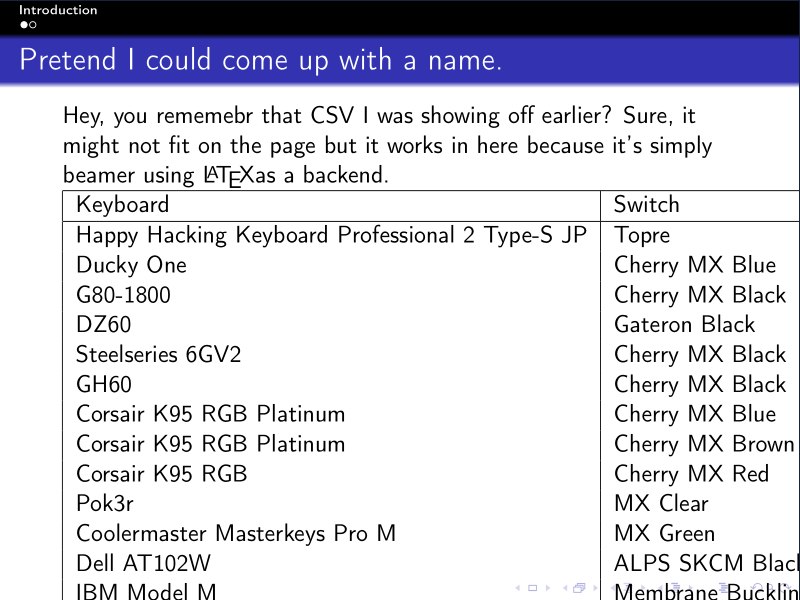
\includegraphics[width=\linewidth]{page2}
	\caption{The second page made with \LaTeX{} and Beamer}
\end{figure}

\begin{figure}[H]
	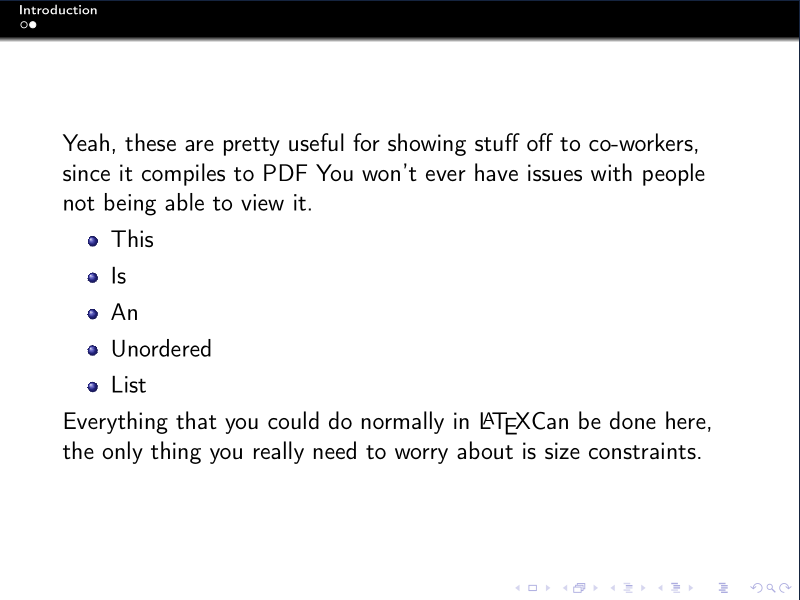
\includegraphics[width=\linewidth]{page3}
	\caption{The third page made with \LaTeX{} and Beamer}
\end{figure}
\end{document}
